\SourceLeaf{363}
\clearpage
\begin{center}[V.]\end{center}
\begin{center}\bfseries ZUR THEORIE DER DREHUNG DER KUGELFLÄCHE IN SICH SELBST.\end{center}

Die Aufgabe, zwei Drehungen in Eine zu vereinigen, kann auf doppelte Weise aufgelöset werden.

I. Man soll die beiden Drehungen, die erste $a$ um den Punkt $A$ und die zweite $\beta$ um den Punkt $B$, in Eine vereinigen.

\begin{center}
\begin{minipage}{4.4cm}\resizebox{4.4cm}{!}{%
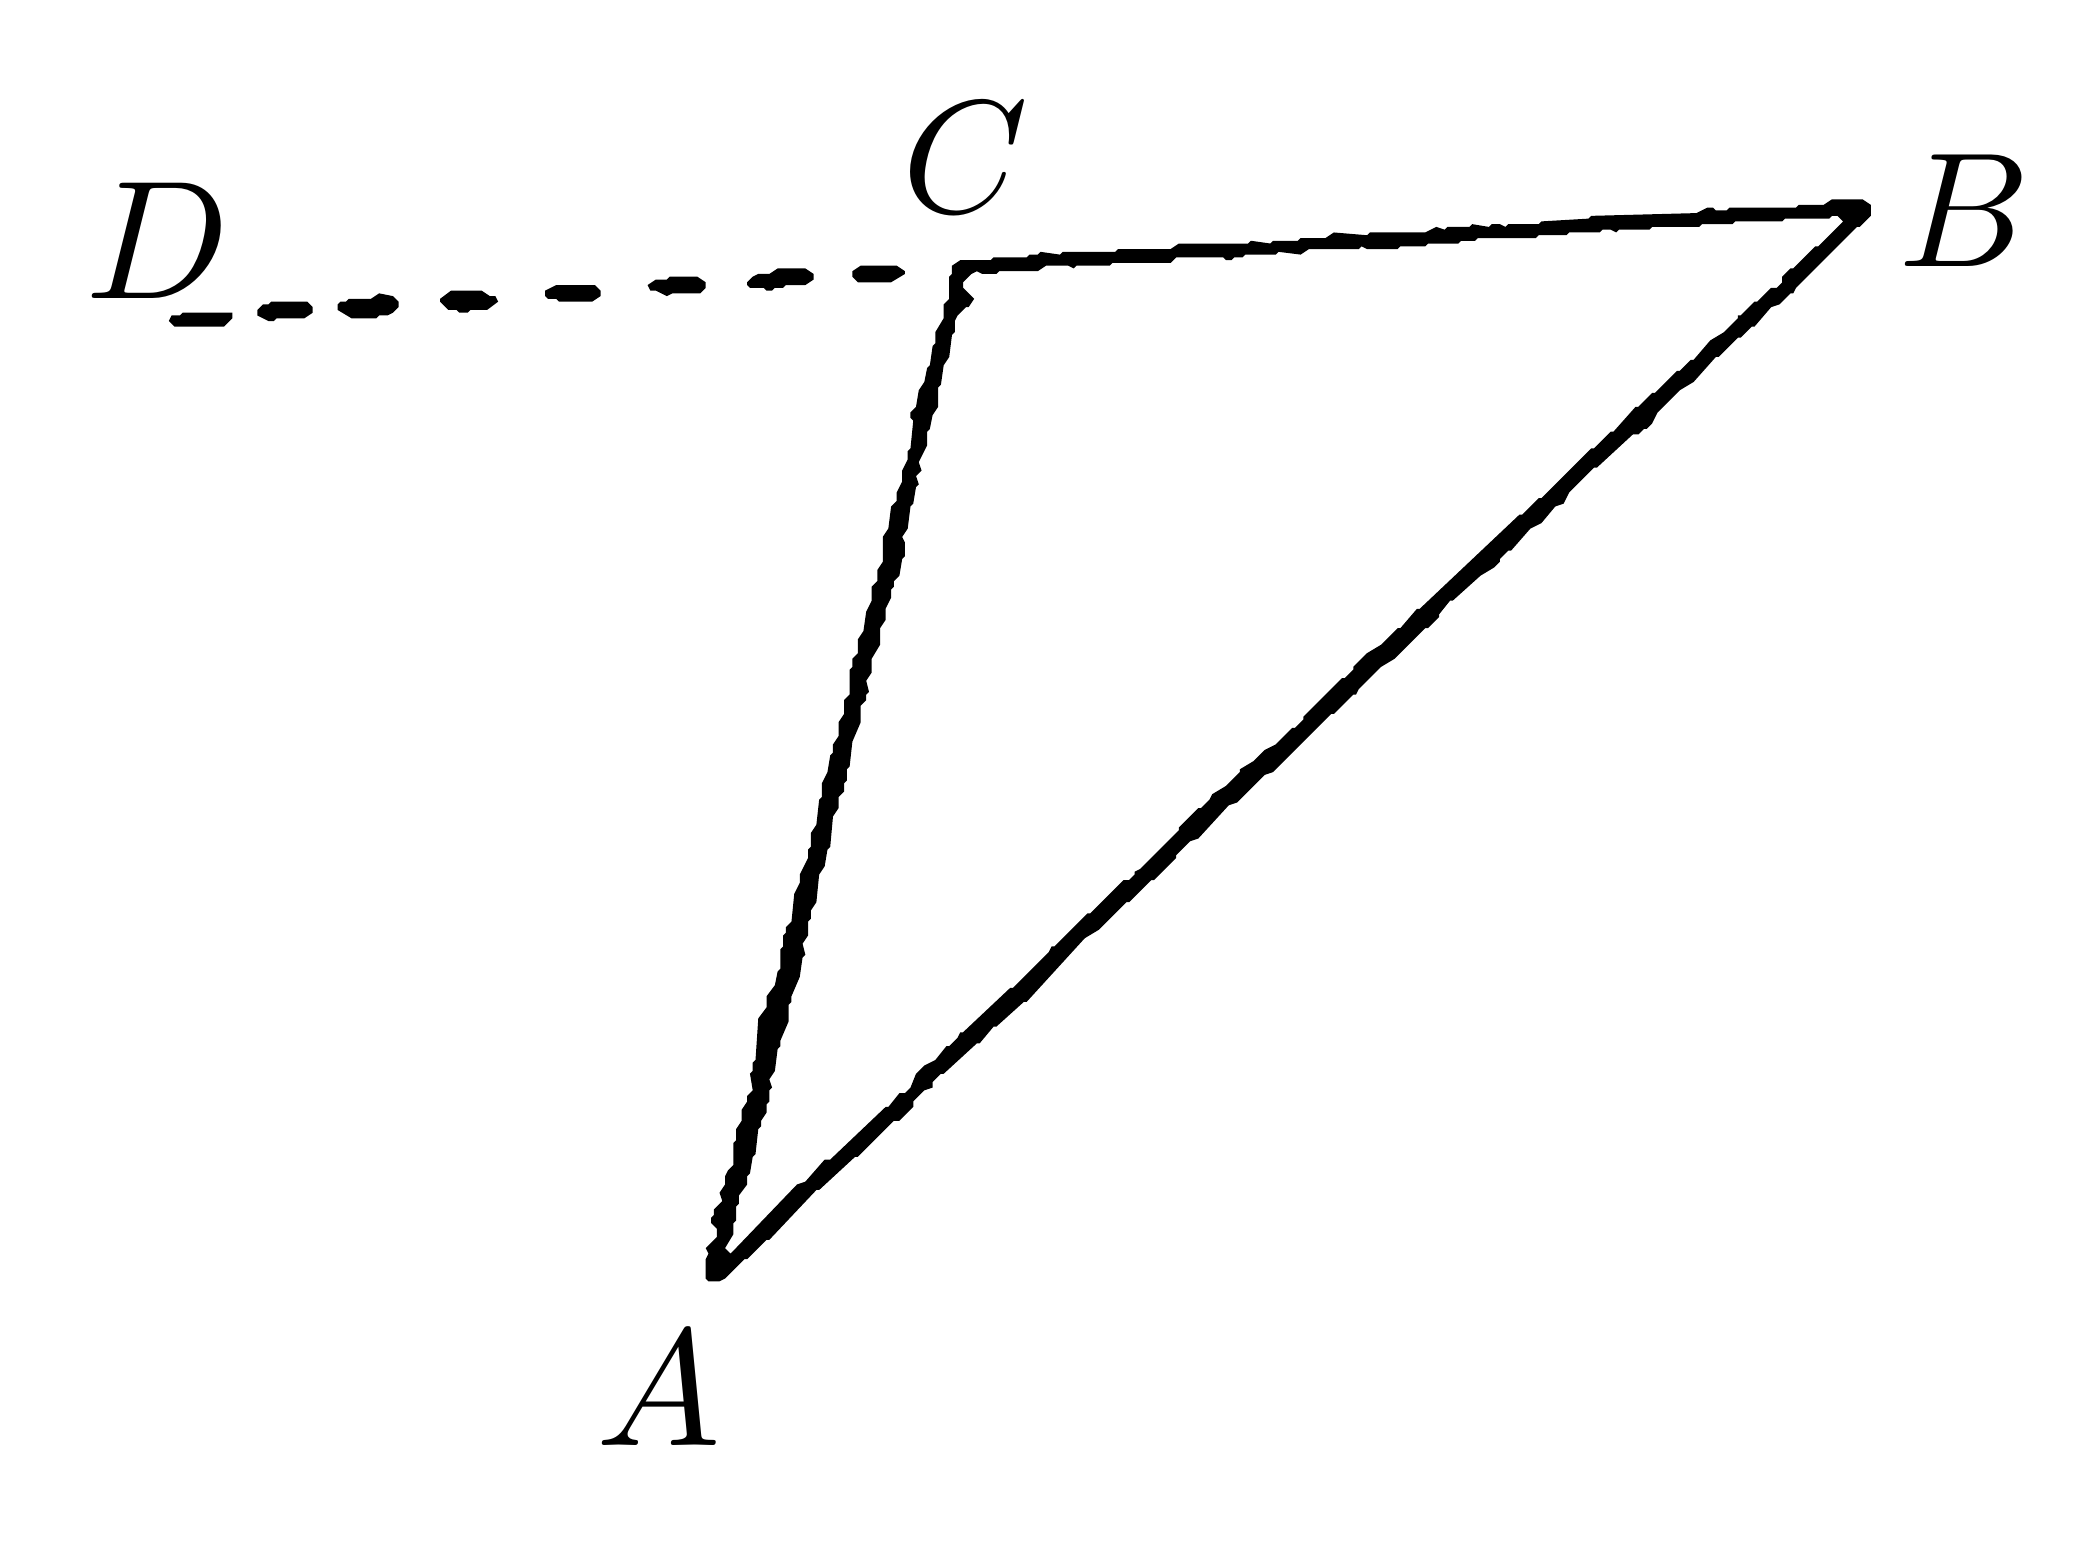
\begin{tikzpicture}[x=1pt,y=-1pt]
\path[use as bounding box] (0,0) rectangle (734,539);
\path[fill=black,draw=none,even odd rule]
(51,106) -- (53,108) -- (71,108) -- (74,105) -- (74,103) -- (56,103) -- (55,104) -- (52,104) -- cycle
(83,102) -- (83,104) -- (87,106) -- (89,106) -- (90,105) -- (100,105) -- (103,103) -- (103,101) -- (101,99) -- (88,99) -- (87,100) -- (85,100) -- cycle
(134,99) -- (132,97) -- (127,96) -- (124,98) -- (116,98) -- (115,99) -- (113,99) -- (112,100) -- (112,102) -- (117,105) -- (126,105) -- (127,104) -- (130,104) -- (132,103) -- (134,101) -- cycle
(149,98) -- (149,99) -- (152,102) -- (155,102) -- (156,103) -- (159,103) -- (160,102) -- (166,102) -- (170,99) -- (169,97) -- (167,97) -- (164,95) -- (153,95) -- cycle
(187,95) -- (187,97) -- (188,98) -- (191,98) -- (192,99) -- (204,99) -- (207,97) -- (207,95) -- (205,93) -- (191,93) -- cycle
(224,93) -- (225,95) -- (227,95) -- (231,97) -- (233,96) -- (243,96) -- (245,94) -- (245,92) -- (242,90) -- (232,90) -- (231,91) -- (227,91) -- cycle
(260,93) -- (261,94) -- (266,94) -- (267,95) -- (269,95) -- (270,94) -- (273,94) -- (274,93) -- (281,93) -- (284,91) -- (284,89) -- (281,87) -- (271,87) -- (268,89) -- (264,89) -- (262,90) -- (260,92) -- cycle
(298,88) -- (298,90) -- (300,92) -- (312,92) -- (317,89) -- (317,88) -- (314,86) -- (301,86) -- cycle
(666,64) -- (663,62) -- (652,62) -- (649,64) -- (640,64) -- (639,65) -- (615,65) -- (614,66) -- (610,66) -- (609,65) -- (607,65) -- (603,67) -- (565,68) -- (564,69) -- (547,70) -- (546,71) -- (535,71) -- (534,72) -- (532,71) -- (529,71) -- (528,72) -- (522,71) -- (521,72) -- (513,72) -- (512,73) -- (509,72) -- (505,74) -- (485,74) -- (484,75) -- (472,74) -- (469,76) -- (460,76) -- (459,77) -- (450,77) -- (449,78) -- (442,77) -- (441,78) -- (416,78) -- (413,80) -- (394,80) -- (393,81) -- (374,81) -- (373,82) -- (366,81) -- (365,82) -- (362,82) -- (361,83) -- (349,83) -- (348,84) -- (337,84) -- (334,86) -- (334,89) -- (333,90) -- (333,98) -- (331,100) -- (331,105) -- (328,110) -- (328,114) -- (327,115) -- (326,122) -- (325,123) -- (324,128) -- (322,131) -- (321,137) -- (319,139) -- (319,141) -- (320,142) -- (319,152) -- (318,153) -- (318,156) -- (316,160) -- (316,164) -- (314,168) -- (314,171) -- (312,173) -- (311,181) -- (309,184) -- (309,193) -- (307,196) -- (307,200) -- (305,202) -- (305,207) -- (303,211) -- (302,218) -- (300,221) -- (300,226) -- (298,228) -- (298,231) -- (297,232) -- (297,241) -- (295,243) -- (295,248) -- (293,251) -- (293,256) -- (291,259) -- (291,262) -- (290,263) -- (289,269) -- (287,273) -- (287,278) -- (286,279) -- (285,288) -- (283,291) -- (283,296) -- (282,297) -- (282,300) -- (279,306) -- (279,309) -- (277,313) -- (276,323) -- (274,325) -- (274,327) -- (273,328) -- (273,332) -- (272,333) -- (272,340) -- (271,341) -- (270,346) -- (267,350) -- (267,354) -- (264,358) -- (263,373) -- (262,374) -- (262,377) -- (261,378) -- (262,384) -- (260,386) -- (260,388) -- (258,391) -- (258,395) -- (256,398) -- (256,402) -- (255,403) -- (255,411) -- (253,413) -- (252,415) -- (252,418) -- (250,421) -- (251,424) -- (248,427) -- (248,429) -- (247,430) -- (247,432) -- (249,434) -- (249,437) -- (245,441) -- (246,443) -- (245,445) -- (245,452) -- (246,453) -- (250,453) -- (252,452) -- (259,445) -- (260,445) -- (267,438) -- (268,438) -- (285,420) -- (286,420) -- (299,408) -- (300,408) -- (313,395) -- (315,395) -- (320,390) -- (320,388) -- (324,384) -- (327,383) -- (327,381) -- (330,378) -- (331,378) -- (343,367) -- (344,367) -- (349,361) -- (350,361) -- (360,352) -- (361,352) -- (382,329) -- (387,326) -- (397,316) -- (398,316) -- (406,308) -- (407,308) -- (415,300) -- (415,299) -- (420,294) -- (423,293) -- (434,281) -- (437,280) -- (447,270) -- (450,269) -- (471,248) -- (472,248) -- (479,241) -- (480,241) -- (481,239) -- (489,231) -- (494,228) -- (505,217) -- (506,217) -- (510,213) -- (510,212) -- (514,207) -- (515,207) -- (525,198) -- (530,195) -- (532,193) -- (532,192) -- (535,189) -- (536,189) -- (543,181) -- (547,179) -- (552,173) -- (555,172) -- (557,168) -- (566,159) -- (567,159) -- (580,147) -- (582,147) -- (584,145) -- (585,145) -- (587,143) -- (589,139) -- (597,131) -- (602,128) -- (610,119) -- (611,119) -- (618,112) -- (619,112) -- (623,108) -- (624,108) -- (630,101) -- (633,100) -- (637,96) -- (638,96) -- (639,94) -- (661,72) -- (662,72) -- (666,68) -- cycle
(656,70) -- (647,79) -- (646,79) -- (638,87) -- (637,87) -- (634,90) -- (634,92) -- (632,94) -- (630,94) -- (625,99) -- (624,99) -- (619,104) -- (618,104) -- (618,105) -- (613,110) -- (608,113) -- (602,120) -- (601,120) -- (597,124) -- (596,124) -- (588,132) -- (587,132) -- (582,137) -- (581,137) -- (573,146) -- (572,146) -- (566,152) -- (565,152) -- (547,170) -- (546,170) -- (540,176) -- (539,176) -- (503,210) -- (502,210) -- (496,217) -- (495,217) -- (489,223) -- (484,226) -- (479,231) -- (479,232) -- (476,235) -- (475,235) -- (461,249) -- (461,250) -- (458,253) -- (457,253) -- (451,259) -- (447,261) -- (443,265) -- (438,268) -- (438,269) -- (433,274) -- (428,277) -- (427,279) -- (424,282) -- (423,282) -- (416,289) -- (416,290) -- (402,304) -- (400,305) -- (400,306) -- (398,308) -- (396,308) -- (384,320) -- (383,320) -- (371,332) -- (370,332) -- (369,334) -- (356,347) -- (355,347) -- (338,363) -- (337,363) -- (336,365) -- (333,368) -- (332,368) -- (328,373) -- (324,375) -- (321,378) -- (319,383) -- (317,385) -- (315,385) -- (311,390) -- (310,390) -- (290,409) -- (288,409) -- (281,417) -- (278,418) -- (254,443) -- (252,441) -- (255,436) -- (255,432) -- (256,431) -- (256,426) -- (257,425) -- (257,422) -- (260,418) -- (260,415) -- (261,414) -- (262,408) -- (263,407) -- (264,398) -- (265,397) -- (265,395) -- (267,392) -- (267,389) -- (268,388) -- (268,384) -- (269,383) -- (268,380) -- (270,377) -- (271,369) -- (272,368) -- (272,366) -- (275,359) -- (275,353) -- (276,352) -- (276,350) -- (279,343) -- (280,336) -- (281,335) -- (280,331) -- (282,328) -- (282,323) -- (283,322) -- (283,319) -- (285,316) -- (286,306) -- (288,303) -- (289,297) -- (290,296) -- (291,285) -- (293,282) -- (293,278) -- (295,276) -- (295,273) -- (296,272) -- (296,268) -- (297,267) -- (298,258) -- (301,251) -- (301,245) -- (303,243) -- (303,241) -- (304,240) -- (303,236) -- (305,233) -- (305,228) -- (308,223) -- (308,217) -- (310,214) -- (310,210) -- (312,206) -- (312,203) -- (313,202) -- (313,200) -- (315,198) -- (316,192) -- (317,191) -- (317,186) -- (316,184) -- (318,181) -- (319,173) -- (320,172) -- (321,166) -- (322,165) -- (321,162) -- (323,160) -- (322,157) -- (325,151) -- (325,146) -- (326,145) -- (327,140) -- (329,137) -- (329,130) -- (330,129) -- (331,122) -- (333,119) -- (334,111) -- (335,110) -- (335,106) -- (336,104) -- (339,101) -- (340,101) -- (342,98) -- (338,94) -- (338,92) -- (341,89) -- (343,88) -- (345,89) -- (350,89) -- (351,88) -- (365,88) -- (368,86) -- (376,86) -- (378,87) -- (379,86) -- (391,86) -- (392,85) -- (413,85) -- (415,83) -- (432,83) -- (433,84) -- (435,84) -- (436,83) -- (439,83) -- (440,82) -- (451,82) -- (452,81) -- (460,82) -- (463,80) -- (481,80) -- (482,79) -- (484,80) -- (495,80) -- (496,79) -- (505,79) -- (506,78) -- (517,78) -- (518,77) -- (523,77) -- (524,76) -- (545,76) -- (546,75) -- (556,75) -- (557,74) -- (568,74) -- (569,73) -- (572,73) -- (574,74) -- (575,73) -- (586,73) -- (587,72) -- (604,72) -- (605,71) -- (616,71) -- (617,70) -- (634,70) -- (635,69) -- (651,69) -- (652,68) -- (654,68) -- cycle;
\node[inner sep=0pt,font=\fontsize{10}{10}\selectfont] at (339,47) {\scalebox{5.8}{$C$}};
\node[inner sep=0pt,font=\fontsize{10}{10}\selectfont] at (700,66) {\scalebox{5.9}{$B$}};
\node[inner sep=0pt,font=\fontsize{10}{10}\selectfont] at (47,77) {\scalebox{6.1}{$D$}};
\node[inner sep=0pt,font=\fontsize{10}{10}\selectfont] at (228,492) {\scalebox{6.0}{$A$}};
\end{tikzpicture}%
}
\end{minipage}\hfill
\begin{minipage}{8.1cm}\raggedright
Man verbinde $AB$; setze
\[
\begin{aligned}
BAC&=-\tfrac12a\quad\text{oder}\quad CAB=+\tfrac12a,\\
ABC&=+\tfrac12\beta,
\end{aligned}
\]
und construire das Dreieck $ABC$. Dann ist $2ACD$ die aus der Verbindung der beiden Drehungen zusammengesetzte.
\end{minipage}
\end{center}

\begin{center}\resizebox{3.2cm}{!}{%
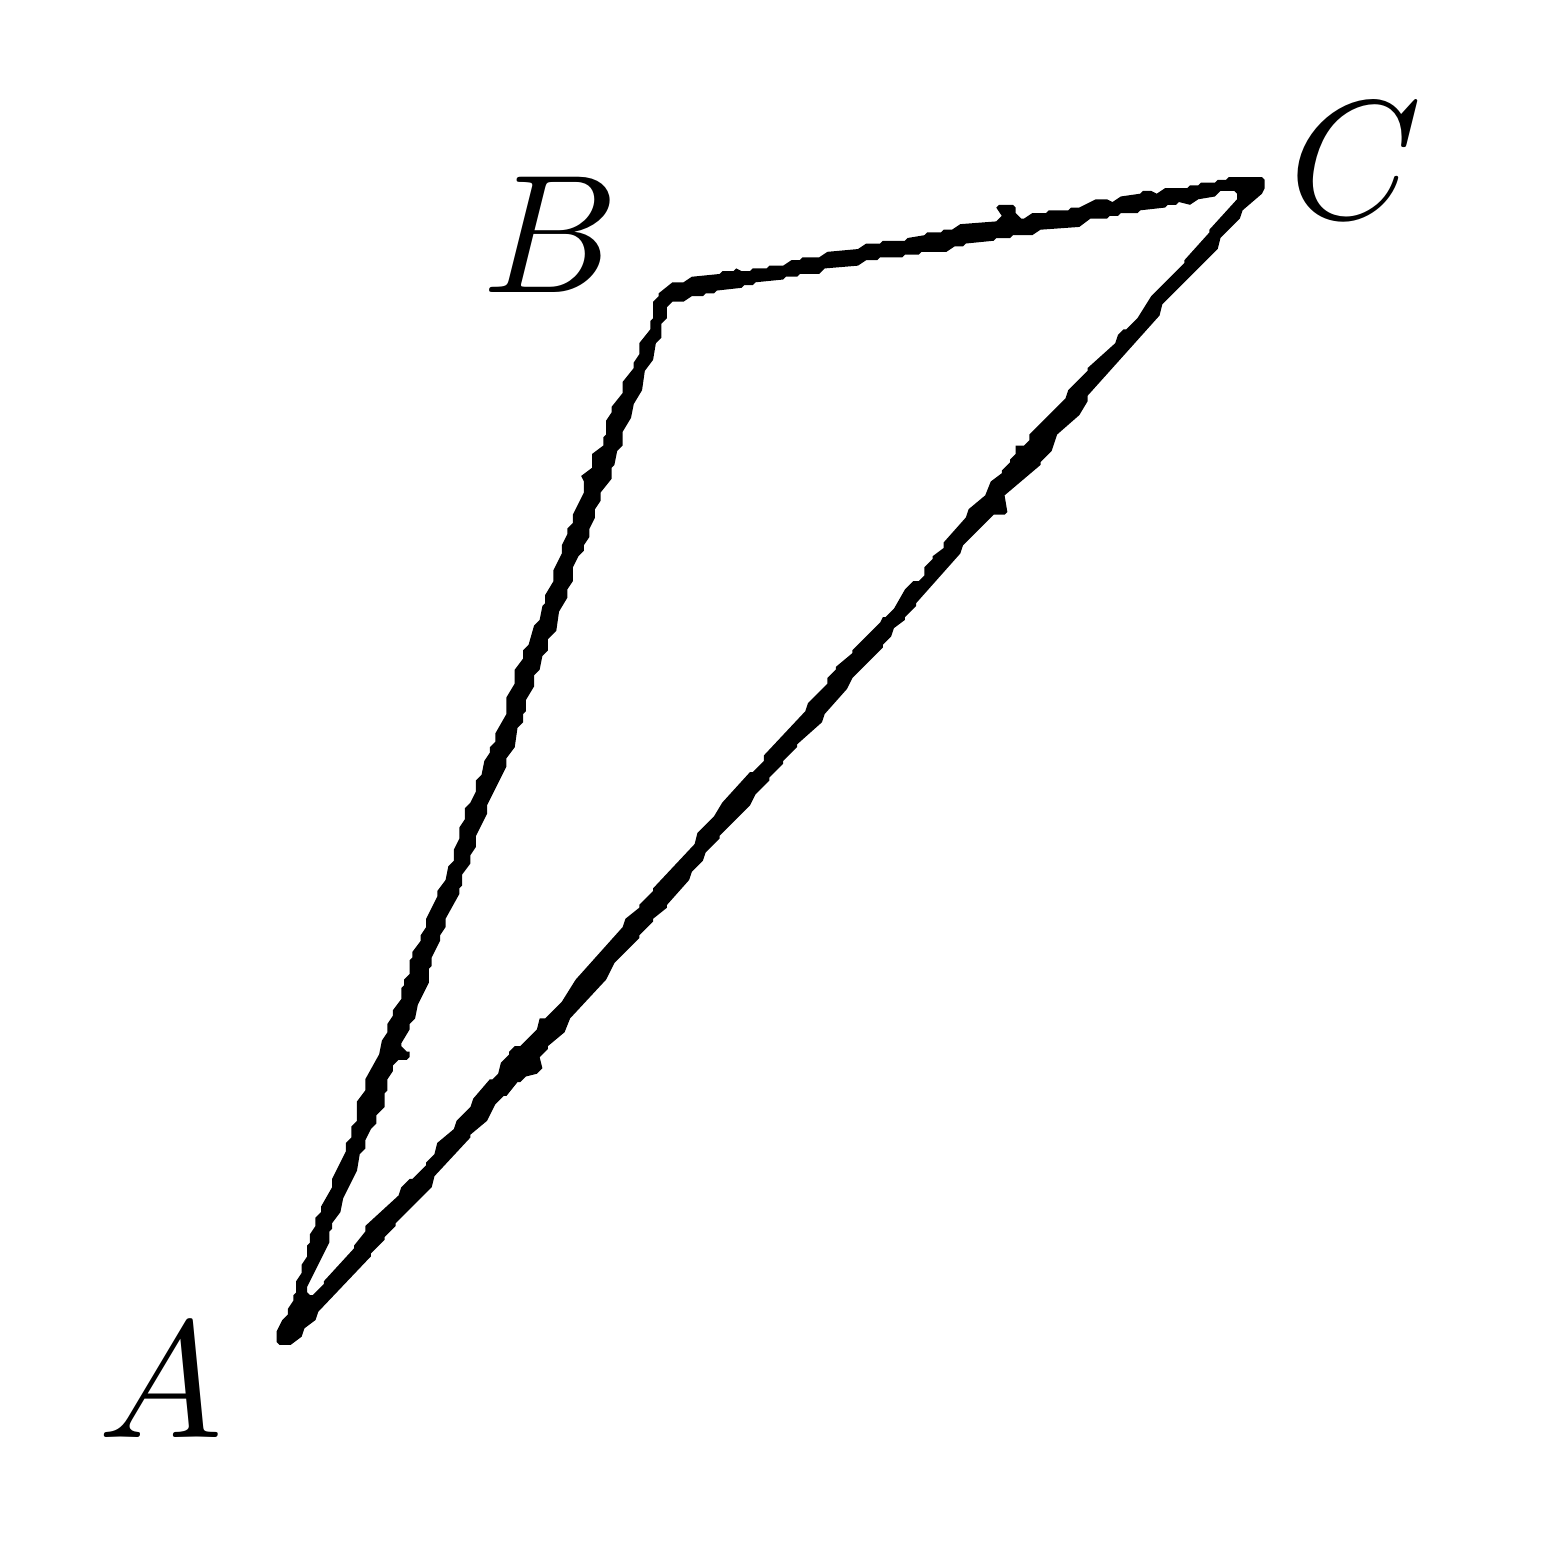
\begin{tikzpicture}[x=1pt,y=-1pt]
\path[use as bounding box] (0,0) rectangle (539,539);
\path[fill=black,draw=none,even odd rule]
(446,54) -- (434,54) -- (433,55) -- (430,55) -- (429,56) -- (424,56) -- (423,57) -- (420,57) -- (419,58) -- (411,58) -- (408,60) -- (406,59) -- (403,59) -- (402,60) -- (395,61) -- (392,63) -- (390,62) -- (386,62) -- (380,65) -- (377,65) -- (376,66) -- (369,66) -- (368,67) -- (363,67) -- (360,69) -- (359,69) -- (357,67) -- (357,65) -- (356,64) -- (351,64) -- (350,65) -- (352,68) -- (350,70) -- (337,71) -- (334,73) -- (331,73) -- (330,74) -- (325,74) -- (324,75) -- (318,76) -- (317,77) -- (309,77) -- (308,78) -- (303,78) -- (300,80) -- (289,81) -- (286,83) -- (280,83) -- (279,84) -- (276,84) -- (273,86) -- (268,86) -- (267,87) -- (262,87) -- (261,88) -- (258,88) -- (256,87) -- (255,88) -- (251,88) -- (250,89) -- (240,90) -- (237,92) -- (233,92) -- (228,96) -- (228,97) -- (226,99) -- (226,105) -- (225,106) -- (225,109) -- (221,114) -- (221,118) -- (219,121) -- (219,123) -- (215,128) -- (215,132) -- (211,137) -- (211,139) -- (209,142) -- (209,147) -- (208,148) -- (208,151) -- (204,154) -- (204,159) -- (200,162) -- (201,164) -- (201,168) -- (197,176) -- (197,179) -- (195,181) -- (195,183) -- (193,187) -- (193,190) -- (190,196) -- (190,200) -- (187,205) -- (187,208) -- (186,209) -- (185,214) -- (183,216) -- (181,223) -- (179,225) -- (179,228) -- (176,232) -- (176,237) -- (173,242) -- (173,248) -- (169,255) -- (169,258) -- (167,260) -- (167,262) -- (165,265) -- (164,270) -- (162,272) -- (162,276) -- (160,280) -- (158,282) -- (158,286) -- (156,289) -- (156,293) -- (154,297) -- (154,301) -- (152,303) -- (151,308) -- (148,312) -- (148,314) -- (144,322) -- (144,325) -- (142,328) -- (142,330) -- (139,334) -- (139,336) -- (138,337) -- (138,342) -- (136,344) -- (136,346) -- (135,347) -- (135,351) -- (132,355) -- (132,357) -- (130,360) -- (130,363) -- (128,366) -- (127,371) -- (122,380) -- (122,384) -- (119,388) -- (119,395) -- (117,397) -- (117,401) -- (115,403) -- (115,406) -- (110,416) -- (110,419) -- (106,426) -- (106,428) -- (104,430) -- (104,433) -- (102,436) -- (102,439) -- (101,440) -- (101,444) -- (99,447) -- (99,450) -- (97,453) -- (97,457) -- (96,458) -- (96,460) -- (94,463) -- (94,465) -- (92,467) -- (90,471) -- (90,475) -- (91,476) -- (95,476) -- (99,473) -- (100,470) -- (104,467) -- (105,464) -- (124,444) -- (124,443) -- (129,438) -- (129,437) -- (133,433) -- (133,432) -- (146,419) -- (147,415) -- (160,401) -- (160,400) -- (166,395) -- (169,389) -- (172,386) -- (173,386) -- (177,381) -- (178,381) -- (180,379) -- (184,378) -- (186,376) -- (185,372) -- (188,369) -- (188,368) -- (194,363) -- (196,358) -- (209,344) -- (212,338) -- (221,329) -- (221,328) -- (226,323) -- (226,322) -- (231,318) -- (231,317) -- (239,308) -- (240,305) -- (244,301) -- (245,298) -- (250,293) -- (250,292) -- (261,281) -- (263,277) -- (268,272) -- (268,271) -- (273,266) -- (273,265) -- (278,260) -- (278,259) -- (287,251) -- (288,248) -- (296,239) -- (298,235) -- (309,224) -- (309,223) -- (312,220) -- (313,217) -- (317,214) -- (317,213) -- (321,209) -- (321,208) -- (337,190) -- (338,187) -- (349,176) -- (353,176) -- (354,175) -- (353,169) -- (366,158) -- (366,157) -- (370,153) -- (372,147) -- (380,140) -- (383,135) -- (383,133) -- (409,104) -- (410,100) -- (430,80) -- (431,76) -- (438,69) -- (439,66) -- (446,60) -- (447,58) -- (447,55) -- cycle
(436,59) -- (437,60) -- (437,62) -- (427,73) -- (427,74) -- (418,84) -- (418,85) -- (406,97) -- (401,105) -- (397,109) -- (396,109) -- (394,111) -- (393,114) -- (383,123) -- (383,124) -- (376,131) -- (375,134) -- (362,147) -- (362,149) -- (360,151) -- (357,151) -- (357,154) -- (355,156) -- (355,157) -- (352,160) -- (352,161) -- (348,164) -- (346,169) -- (340,174) -- (339,177) -- (331,186) -- (331,188) -- (327,191) -- (327,192) -- (324,195) -- (324,198) -- (322,200) -- (320,200) -- (317,203) -- (313,210) -- (310,213) -- (309,213) -- (308,215) -- (298,225) -- (298,226) -- (292,231) -- (292,232) -- (289,235) -- (289,237) -- (282,244) -- (281,247) -- (266,263) -- (266,265) -- (262,269) -- (261,269) -- (251,280) -- (248,285) -- (242,291) -- (241,295) -- (226,311) -- (226,312) -- (221,317) -- (221,318) -- (216,322) -- (215,325) -- (198,344) -- (193,352) -- (187,358) -- (185,358) -- (184,362) -- (178,368) -- (176,368) -- (174,370) -- (174,371) -- (171,374) -- (170,378) -- (168,380) -- (167,380) -- (161,387) -- (160,390) -- (155,395) -- (154,398) -- (148,403) -- (147,407) -- (144,410) -- (144,411) -- (139,416) -- (138,416) -- (135,419) -- (134,422) -- (122,433) -- (122,435) -- (118,440) -- (118,441) -- (107,453) -- (107,454) -- (103,458) -- (102,458) -- (101,457) -- (101,455) -- (109,439) -- (109,435) -- (110,434) -- (110,432) -- (113,428) -- (114,423) -- (119,413) -- (120,407) -- (122,405) -- (122,402) -- (124,398) -- (126,396) -- (126,393) -- (129,390) -- (129,385) -- (130,384) -- (130,380) -- (132,377) -- (132,375) -- (134,373) -- (137,373) -- (138,372) -- (138,370) -- (137,370) -- (135,368) -- (135,367) -- (138,362) -- (138,360) -- (140,358) -- (141,353) -- (145,345) -- (145,340) -- (146,339) -- (146,336) -- (149,330) -- (149,328) -- (151,325) -- (151,322) -- (156,313) -- (156,311) -- (157,310) -- (157,306) -- (160,302) -- (160,299) -- (162,296) -- (162,292) -- (166,284) -- (166,281) -- (173,267) -- (173,264) -- (176,260) -- (177,253) -- (179,251) -- (179,248) -- (180,247) -- (180,243) -- (183,238) -- (183,234) -- (185,232) -- (186,227) -- (188,225) -- (188,221) -- (191,218) -- (192,211) -- (195,206) -- (195,203) -- (197,200) -- (197,195) -- (199,191) -- (201,189) -- (201,187) -- (203,184) -- (203,181) -- (205,177) -- (205,174) -- (207,171) -- (207,168) -- (211,163) -- (211,159) -- (212,158) -- (213,153) -- (215,151) -- (215,146) -- (218,141) -- (219,136) -- (222,131) -- (223,124) -- (226,120) -- (227,114) -- (229,112) -- (229,107) -- (231,105) -- (231,101) -- (233,99) -- (237,99) -- (240,97) -- (244,97) -- (245,96) -- (248,96) -- (249,95) -- (258,94) -- (259,93) -- (262,93) -- (263,92) -- (273,91) -- (274,90) -- (278,90) -- (279,89) -- (286,89) -- (288,87) -- (300,86) -- (303,84) -- (307,84) -- (308,83) -- (316,83) -- (317,82) -- (322,82) -- (323,81) -- (332,81) -- (335,79) -- (338,79) -- (339,78) -- (349,77) -- (350,76) -- (355,76) -- (356,75) -- (363,75) -- (366,73) -- (380,72) -- (384,69) -- (390,69) -- (391,68) -- (394,68) -- (395,67) -- (401,67) -- (402,66) -- (411,65) -- (412,64) -- (415,64) -- (416,63) -- (420,64) -- (423,62) -- (429,61) -- (431,59) -- cycle;
\node[inner sep=0pt,font=\fontsize{10}{10}\selectfont] at (480,48) {\scalebox{6.1}{$C$}};
\node[inner sep=0pt,font=\fontsize{10}{10}\selectfont] at (189,75) {\scalebox{6.1}{$B$}};
\node[inner sep=0pt,font=\fontsize{10}{10}\selectfont] at (48,489) {\scalebox{6.0}{$A$}};
\end{tikzpicture}%
}
\end{center}
II. Anstatt Drehungen um Punkte betrachte man Schiebungen längs grössten Kreisen.

Dann ist die Schiebung $2AC$ aus $2AB$ und $2BC$ zusammengesetzt.

\Needspace{10\baselineskip}
\begin{center}\bfseries BEMERKUNGEN.\end{center}

Die vorstehenden Notizen [I], [II] und [III] stehen in einem Handbuche. Die folgende Notiz [IV] befindet sich auf einem einzelnen Zettel ohne Datirung. Sie zeigt, dass \textsc{Gauss} den Zusammenhang der linearen Substitutionen einer complexen Veränderlichen mit den Drehungen der Kugelfläche in sich selbst erkannt hatte. Aus diesem Grunde ist die Notiz [V], die sich auf denselben Gegenstand bezieht, jedoch in rein geometrischer Behandlungsweise, hinzugefügt worden; sie findet sich in einem andern Handbuche und ist vermuthlich schon vor 1819 niedergeschrieben worden.
\begin{flushright}\textsc{Stäckel.}\end{flushright}
